\documentclass[aspectratio=169,11pt]{beamer}
\usepackage[T1]{fontenc}
\usepackage{lmodern,amsmath,amssymb,booktabs,graphicx}
\definecolor{navy}{RGB}{12,30,50}
\definecolor{paper}{RGB}{240,244,249}
\definecolor{accent}{RGB}{83,163,228}
\definecolor{muted}{RGB}{175,194,213}
\setbeamercolor{background canvas}{bg=navy}
\setbeamercolor{normal text}{fg=paper,bg=navy}
\setbeamercolor{frametitle}{fg=paper}
\setbeamercolor{structure}{fg=accent}
\setbeamercolor{footline}{fg=muted,bg=navy}
\setbeamerfont{frametitle}{size=\LARGE,series=\mdseries}
\setbeamertemplate{navigation symbols}{}
\setbeamersize{text margin left=7mm,text margin right=7mm}
\setbeamertemplate{footline}{\hspace{7mm}\scriptsize GROUP 7\quad PUMA 560\hfill\insertframenumber\hspace{7mm}\vspace{3mm}}
\setbeamertemplate{itemize item}{\small\textbullet}
\setlength{\emergencystretch}{2em}
\graphicspath{{assets/}}
\newcommand{\figurefit}[1]{\includegraphics[width=\linewidth,height=.66\textheight,keepaspectratio]{#1}}
\title{PUMA 560 Robot Manipulator}
\author{Satyanarayana \and Sarvajith \and Sathwik \and Sreyas}
\date{Group 7}
\begin{document}

{\usebackgroundtemplate{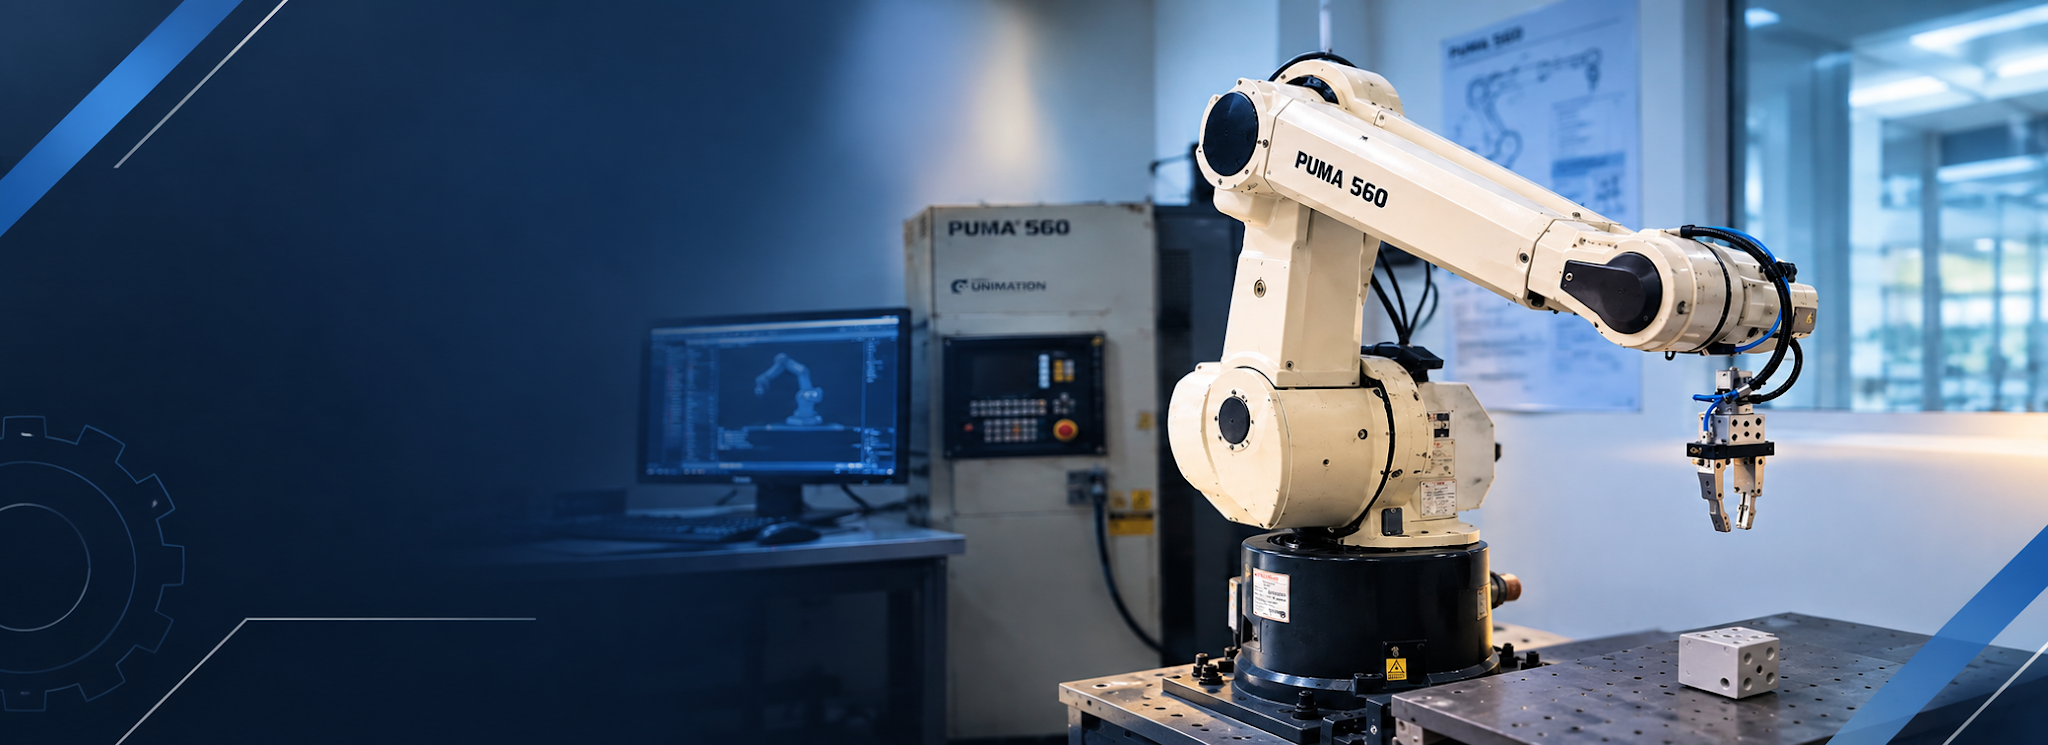
\includegraphics[width=\paperwidth,height=\paperheight]{image1.png}}
\begin{frame}[plain]
\vspace{7mm}
{\large GROUP 7}\par\vspace{8mm}
{\Huge PUMA 560 Robot\par Manipulator}\par\vspace{9mm}
Satyanarayana\par Sarvajith\par Sathwik\par Sreyas
\end{frame}}

\begin{frame}{Project scope}
{\large\color{accent}PUMA560: A six revolute joint manipulator with a spherical wrist}
\vspace{6mm}
\begin{itemize}\setlength\itemsep{5mm}
\item Robot specification and standard DH frames
\item Forward and analytical inverse kinematics
\item Velocity kinematics and singularity analysis
\item Independent checks against MuJoCo
\end{itemize}
\end{frame}

\begin{frame}{Robot geometry and reference frames}
\begin{columns}[c]
\begin{column}{.40\textwidth}
$O_0$: mounting plane\par\medskip
$O_1$: $0.67183\,\mathrm{m}$ above $O_0$\par\bigskip
$O_4=O_5=O_6$: wrist centre\par\medskip
$O_E$: $0.04\,\mathrm{m}$ along $z_6$ from the wrist centre
\end{column}
\begin{column}{.57\textwidth}\figurefit{image2.png}\end{column}
\end{columns}
\end{frame}

\begin{frame}{Standard Denavit--Hartenberg model}
\[ A_i=R_z(q_i)\,T_z(d_i)\,T_x(a_i)\,R_x(\alpha_i) \]
\centering
\begin{tabular}{ccrrr}\toprule
Joint & $\theta$ & $d$ (m) & $a$ (m) & $\alpha$ (deg)\\\midrule
1 & $q_1$ & 0.67183 & 0 & 90\\
2 & $q_2$ & 0 & 0.4318 & 0\\
3 & $q_3$ & 0.15005 & 0.0203 & -90\\
4 & $q_4$ & 0.4318 & 0 & 90\\
5 & $q_5$ & 0 & 0 & -90\\
6 & $q_6$ & 0 & 0 & 0\\\bottomrule
\end{tabular}
\par\medskip{\color{accent}Flange transform: $T_{6E}=\operatorname{Trans}(z,0.04\,\mathrm{m})$}
\end{frame}

\begin{frame}{Forward kinematics}
\begin{columns}[c]
\begin{column}{.40\textwidth}
\[T_{0E}=A_1A_2A_3A_4A_5A_6T_{6E}\]
Input: six joint angles\par\medskip
Output: end-effector pose, all DH frames and wrist centre\par\bigskip
The MuJoCo pose provides an independent comparison
\end{column}
\begin{column}{.57\textwidth}\figurefit{image3.png}\end{column}
\end{columns}
\end{frame}

\begin{frame}{Reachability and joint limits}
\begin{columns}[c]
\begin{column}{.43\textwidth}
\small
\(r\geq |d_3|=0.15005\,\mathrm{m}\)\par\smallskip
\( |a_2-L|\leq\rho\leq a_2+L \)\par\smallskip
\( L=\sqrt{a_3^2+d_4^2} \)\par\smallskip
Outer planar reach: $0.8641\,\mathrm{m}$\par\medskip
\centering
\begin{tabular}{crr}\toprule
Joint & Min (${}^\circ$) & Max (${}^\circ$)\\\midrule
J1 & -160 & 160\\ J2 & -45 & 225\\ J3 & -225 & 45\\
J4 & -110 & 170\\ J5 & -100 & 100\\ J6 & -266 & 266\\\bottomrule
\end{tabular}
\end{column}
\begin{column}{.54\textwidth}\figurefit{image4.png}\end{column}
\end{columns}
\medskip\small A reachable target can still violate every joint-limit branch
\end{frame}

\begin{frame}{Velocity kinematics}
\begin{columns}[c]
\begin{column}{.42\textwidth}
\[\begin{bmatrix}v\\\omega\end{bmatrix}=J(q)\dot q\]
\[J_{v,i}=z_{i-1}\times(p_E-p_{i-1})\]
\[J_{\omega,i}=z_{i-1}\]
Inverse velocity: pseudoinverse or damped least squares
\end{column}
\begin{column}{.55\textwidth}\figurefit{image5.png}\end{column}
\end{columns}
\end{frame}

\begin{frame}{Singularity conditions}
\[\det J=a_2 X\bigl(a_3\sin q_3+d_4\cos q_3\bigr)\sin q_5\]
\vspace{2mm}
\textcolor{accent}{Shoulder: $X=0$}\par
Wrist centre reaches the cylinder about the waist axis\par\medskip
\textcolor{accent}{Elbow: $a_3\sin q_3+d_4\cos q_3=0$}\par
Stretched configuration within limits: $q_3\approx-87.3^\circ$\par\medskip
\textcolor{accent}{Wrist: $\sin q_5=0$}\par
Joint 4 and joint 6 axes align. Within limits: $q_5=0^\circ$
\end{frame}

\begin{frame}{Singular configurations}
\centering
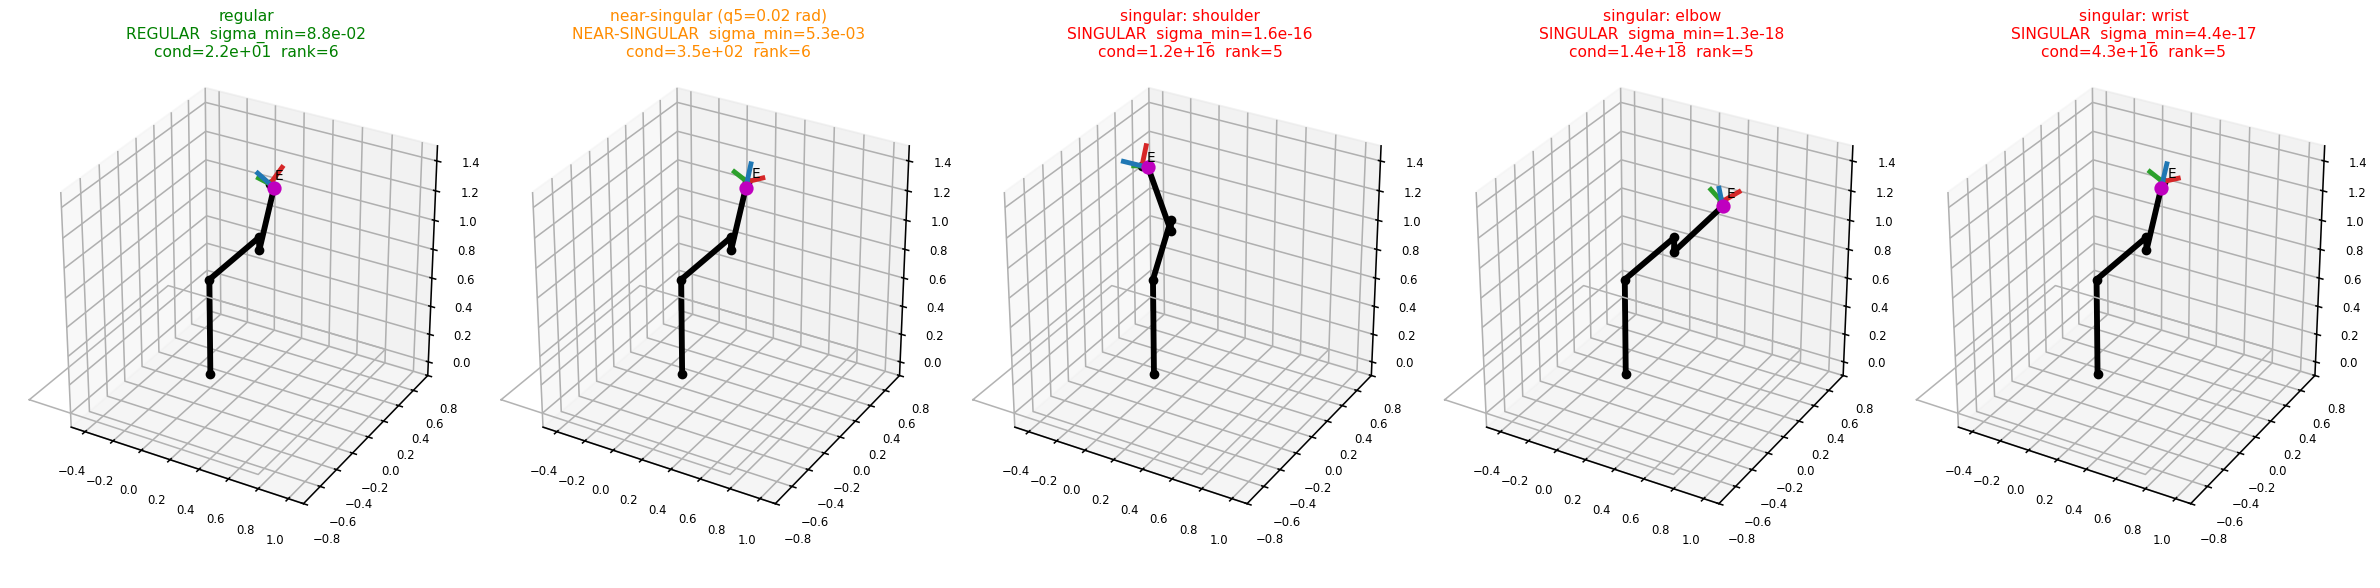
\includegraphics[width=\linewidth,height=.62\textheight,keepaspectratio]{image6.png}
\par\medskip
The Jacobian loses rank and at least one twist direction becomes unavailable
\end{frame}

\begin{frame}{Near-singular joint speeds}
\begin{columns}[c]
\begin{column}{.40\textwidth}
For the weakest twist:
\[\|\dot q\|=\frac{\|\text{twist}\|}{\sigma_{\min}}\]
At $q_5=0.0001\,\mathrm{rad}$:\par\medskip
Pseudoinverse: about $37{,}500\,\mathrm{rad/s}$\par\bigskip
Damping bounds joint speed at the cost of task error
\end{column}
\begin{column}{.57\textwidth}\figurefit{image7.png}\end{column}
\end{columns}
\end{frame}

\begin{frame}{Interactive MuJoCo demonstration}
\begin{columns}[c]
\begin{column}{.39\textwidth}
\begin{itemize}\setlength\itemsep{5mm}
\item Joint-angle or Cartesian input
\item DH frames and IK branch overlays
\item Velocity ellipsoid and arrows
\item Singularity indicator
\end{itemize}
\end{column}
\begin{column}{.58\textwidth}\figurefit{image8.png}\end{column}
\end{columns}
\end{frame}

\begin{frame}{Numerical verification results}
\small\centering
\renewcommand{\arraystretch}{1.65}
\begin{tabular}{p{.28\textwidth}p{.19\textwidth}p{.43\textwidth}}\toprule
Check & Sample size & Reported result\\\midrule
FK vs MuJoCo & 2,000 poses & Max position error $6.8\times10^{-16}\,\mathrm{m}$\\
IK round trip & 3,000 poses & 3,000 / 3,000 recovered\\
Jacobian vs differences & 1,000 poses & Max absolute error $2.6\times10^{-10}$\\
Determinant formula & Report check & Max difference $1.2\times10^{-16}$\\\bottomrule
\end{tabular}
\par\bigskip\raggedright
Boundary, unreachable and singular targets also have dedicated checks
\end{frame}

\begin{frame}{Conclusions and limitations}
\begin{itemize}\setlength\itemsep{9mm}
\item DH forward kinematics agrees with the MuJoCo reference
\item The Jacobian explains lost motion and large joint speeds
\item Future work: dynamics, control and obstacle avoidance
\end{itemize}
\end{frame}

\begin{frame}{References and project sources}
\textcolor{accent}{Project implementation and verification}\par\medskip
\texttt{README.md}, \texttt{src/}, \texttt{run\_all.py}\par
\texttt{results/verification\_report.md}\par\bigskip
\textcolor{accent}{Robot parameters}\par\medskip
Corke and Armstrong-Helouvry (1994)\par\medskip
Armstrong, Khatib and Burdick (1986)\par\medskip
ARTE and rtb-data: \texttt{models/LICENSE\_NOTICE.md}
\end{frame}
\end{document}
